\section{Task Analysis}

We investigated the design needs for collaborative information analysis in three ways. First, we examined existing works that already conducted empirical user studies of information analysts, particularly the works by \citep{Chin2009,Carroll2013,Pirolli2005, Kang2012,Kang2012d}. These works summarize the design needs for supporting collaboration and analytics, as well as empirical user data in support of their arguments. Among them, we used the works by Carroll and his colleagues \citep{Carroll2013,Borge2012,Borge2014} as the most important guidelines because their paper prototype study context was most close to our study. In their study, they observed 22 teams investigating a crime scenario using paper and pen. Teams of participants spent four hours analyzing 222 propositions embedded in a set of problem documents. This study sheds light on team process patterns, collaboration breakdowns, and possible technical support teams need. We reused their experiment materials in our second user study.

We worked closely with the Red Cell Analytics Lab at Pennsylvania State University for over one year. The lab is an instructor-directed student club that is designed to give students experience in analyzing real-world problems to prepare students for the professional world by helping them develop structured analysis skills and critical thinking capabilities. We worked with a fresh student analyst who had just begun to learn the skills and two senior analysts who had more than two years of experience. We met about once every two weeks, observing what and how they performed analytics and having informal interviews in terms of why and pain points.  We also talked to the lab director, Colonel Jake Graham, who had rich in-person experience in professional intelligence analysis before retirement and now a professor teaching analytic skills at Pennsylvania State University. 

We also observed an intelligence analysis course instructed by Colonel Jake Graham. The course  In the course, students learned theories of analysis (e.g. bottom-up analysis vs. top-down analysis, and concepts of hypothesis, assumption, and evidence), analytic techniques (e.g. Analysis of Competing Hypotheses (ACH) \citep{Heuer1999} and Link Analysis \citep{Sparrow1991}), as well as the state-of-the-art tools to support the implementation of those techniques (e.g. PARC ACH \citep{PARC} and Analyst’s Notebook \citep{IBM}. Below we summarized our findings.

\subsection{Major activities: data annotation, data analysis, and hypothesis development}

On a high level, we observed three categories of activities: data modeling, data analysis, and hypothesis generation. A typical workflow is shown in Figure~\ref{fig:workflow}. Analysts received a collection of documents periodically. The documents included police reports, social media collections, news reports, video summaries, and other textual data. Analysts must extract useful information from these documents, connect these pieces of information, make hypotheses of event indicators and warnings. 

\begin{figure}
	\centering
	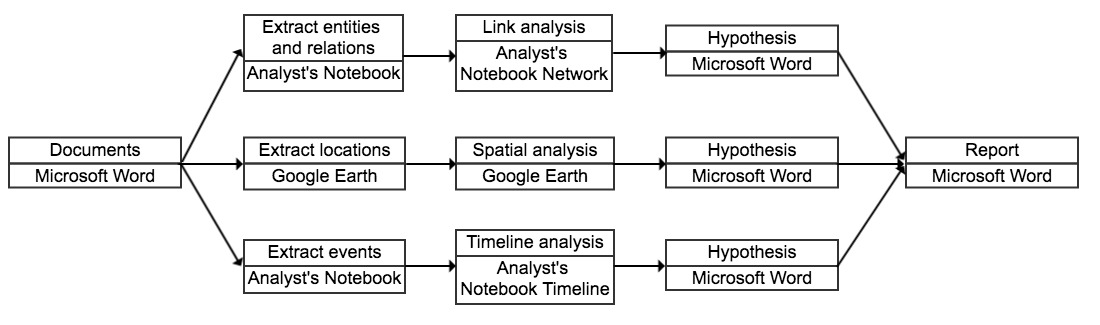
\includegraphics[width=\columnwidth]{./03-System/img/workflow2.jpg}
	\caption{Participant reported intelligence analysis workflow\label{fig:workflow}}
\end{figure}

Upon receiving the documents, analysts would read through and mark critical information. When with pen and paper, they highlighted text and made annotations. They would extract these items and organize them in an ``Information Extraction and Weighting'' table (\ref{tbl:iew_table}). In the table, they investigated each item's face value and alternative value against analytic problems. When with computer support, they created ``entities'' in i2 Analyst's Notebook, a popular software product by IBM for data analysis and investigation. These entities were data objects that described critical attributes and properties. Analysts connected these entities by marking relationships between them. Some frequently seen relationships included ownership, organizational belonging, and phone contact. Location was a special type of entity. To represent the spatial information, analysts replicated the location entities in Google Earth. One interesting detail was that analysts manually exported the location icons used in Analyst's Notebook and imported them into Google Earth. The purpose was to keep consistent the representations in different tools. 

\begin{table}
	\caption{Sample Information Extraction and Weighting table}
	\label{tbl:iew_table}
	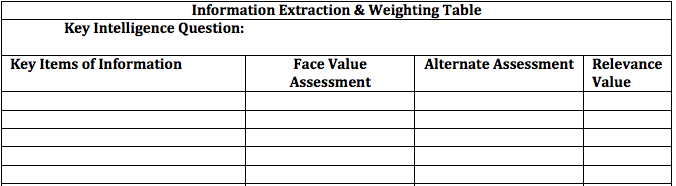
\includegraphics[width=\columnwidth]{./03-System/img/IEW_table.png}
\end{table}

Another special entity type was ``event'', which included a temporal attribute. Event time was important for sequence analysis. Analysts added the start time and the end time of an event, and the repeated date and time if it was a recurring event. 

With the modeled data, analysts tried to find connections and patterns through data visualization. They made use of Analyst's Notebook network tool to map out the entities and their relationships. The timeline tool in Analyst's Notebook displayed the sequential relationship and overlaps between events. They also used Google Earth and identified spatial relationships among events.  To share and keep record of supporting views, they took screenshots and saved in a Microsoft Word document as evidence files. 

Based on these evidence files, analysts generated and recorded hypotheses. These hypotheses are in form of text, but often refer to supporting evidence, either an entity or a visualization of relationships between entities. To compare hypotheses, they often employed the technique of Analysis of Competing Hypotheses (ACH). ACH lays out a full set of hypotheses and examines each item of evidence of its diagnostic value against each hypothesis. Analysts sought evidence to refute hypotheses and picked the least unlikely one. The final delivery was an intelligence report, in which analysts composed their hypothesis and all supporting evidence.

Note that we describe the three activities in a linear fashion for the sake of writing, but analysis could be performed in any order, and most commonly, in an iterative approach.

One problem in the workflow is a breakdown between activities. Systems that support intelligence analysis are aimed at a single activity and therefore only support part of the overall analysis workflow. This imposes a clear boundary between each of these activities on the analysts. For example, IEW helps structure evidence modeling, but does not extend the utilization of evidence to hypothesis generation; ACH assumes that data has been modeled, and that relevant evidence can be adduced appropriately to various hypotheses, but provides no structured support for either. The unintended boundary between phases has the consequence that data modeled in one software cannot be effectively utilized in hypothesis development in another system. And analysts have to handoff, often via replicating the data in the new system, information between software systems, making it difficult to revisit and revise the data model.


\subsection{Collaboration}

Intelligence analysis is fundamentally a collaborative activity because the task can easily become complicated enough that no single individual could handle it. Collaborative intelligence analysis then becomes not only a mental process, but also a group process that involves the management of team resources (tooling, teammate expertise, etc.), teammate goals and motivations, and partner's contemporary and past activities.

Most tools supporting intelligence analysis, however, are not designed for collaborative use. We observed several pain points in participants’ collaboration. For example, participants were unable to contribute simultaneously. Working on the same file would cause conflict. Collaborators had to wait when one teammate was working on the tool. This was known as production blocking \citep{Diehl1987a}, in which individual performing a task became a bottleneck of the team process. To work around the issue, participants often divided their work by tools: each person picked a tool and then created and analyzed an artifact with the tool on their own. This had the consequence that findings and hypotheses be made without integrating collective efforts and diverse knowledge. Participants shared their findings only after they already had a conclusion, which was obviously opposed to collaboration.

Analysts coordinated work outside the tool, by manually sharing documents or graphs through email or cloud storage service (e.g.~Dropbox). As shown in Figure~\ref{fig:workflow}, analysts manually took screenshots of views and copied them into Microsoft Word. This has the consequence that multiple views exist in distributed locations, adding a burden to the analyst’s limited cognition. Analysts could easily overlook certain aspect when they were evaluating hypotheses. The interactive views become static images, making it impossible for collaborators to further explore. Worse, if the data model changes, analysts must manually update the views, resulting in multiple versions of views.